
\documentclass[12pt,a4]{article}
%\documentclass[10pt,twocolumn]{article}
%\documentclass{ecai2010}

\usepackage{graphicx}
\usepackage{epsfig}
\usepackage{latexsym}
\usepackage{url}
\newcommand{\HRule}{\rule{\linewidth}{0.5mm}}

\begin{document}

\begin{titlepage}

\begin{center}


% Upper part of the page

\includegraphics[width=0.49\textwidth]{figure/title}

\textsc{\LARGE King's College London}\\[0.8cm]

\textsc{\Large Final Report}\\[0.4cm]


% Title
\HRule \\[0.2cm]
{ \huge \bfseries  Oasis}\\[0.2cm]

\HRule \\[0.6cm]

% Author and supervisor

\large
\emph{Author:}\\[0.2cm]
Tehao \textsc{Ye}\\
Zhihao \textsc{Zhu}\\
Jiawei \textsc{Zhou}\\
Yankai \textsc{Chen}\\
Yibo \textsc{Liu}\\
Mohan \textsc{Chi}\\
Jiawei \textsc{Ding}\\[0.8cm]


% Bottom of the page
{\large \today}

\end{center}
\end{titlepage}
\clearpage
\tableofcontents
\clearpage
\section{Introduction}\label{Introduction}
With the develop of computing capacity, the File synchronization become a common tool for both individuals and companies. Moreover, the portable device like smartphone and tablet PC play an important role nowadays, and file storage in these portable devices has become a common problem for users. The File synchronization not only let user to store data across the different platforms but also gives users a more security way to store their data and prevent from losing data. Last but not least, the method for file comparison such as how to deal with conflict files or version conflict is a key for a File synchronization, and we treat this as a fundamental problem for our project.\\
\\
Our project name is Onebox, which aims to build a multi-host file synchronization tool which can transmit files across multiple platforms. The main features of it are  uploading and downloading different types and sizes, file comparison and comparing files. Moreover, we also add online streaming and version control in order to strength usability. Users can access it by Android application or web browser.  HTTP protocol are used for Android App and Web APP to download and upload files. Bootstrap and Angular are used for front-end development of Web App. We tried to make a suitable solution for file synchronization system and execute all core functions as requirements. In the end, we made some achievements and completed this project, and we also learned some value experience throughout this project.


\section{Review}\label{Section-Frameworks}
Due to the limitation of local storage and security concerns, the File synchronization develop rapidly these years both in commercial and domestic fields. Dropbox and OneDrive, along with Google Drive, are the big three of the cloud storage market for SMBs and enterprises[1]. Moreover, Box are also famous in cloud storage market. Although the main function may be the same among these application, there are still some function differences. Before we started our project, we compare Dropbox, OneDrive and Google Drive in three different dimension.
\subsection{Free Storage Cloud}\label{SubSec-Value}	
All users of these companies enjoy free cloud storage, but Google Drive users have comparative large free storage than the others, which is 15GB. OneDrive and Dropbox have 5GB and 2GB free storage cloud for users respectively. Moreover, all companies also offer paid storage for users. 

\subsection{Paid Storage}\label{SubSec-Value}	
OneDrive has most generous offer to its customers, which 1.99 per month to increase 50 GB storage. In the other way, The per month cost for  Google Drive and Dropbox is 10 USD. Users of Google Drive will enjoy 1TB by paying 10 USD per month, but Dropbox user can only enjoy 100GB by paying same amount.

\subsection{Characteristic features}\label{SubSec-Value}	
Besides storage cloud, we mainly focus characteristic features among these app. As for OneDrive, it focus on Windows and Office integration, and users can easily access and edit Office documents by using OneDrive. As for the Dropbox, well performance across different platform would be its characteristic feature. Moreover, Dropbox has more sophisticated file comparison, and it retains file history version for each file and user can restore to early revising file version anytime[2]. As for Google Drive, users would be able to share there files easily, and online collaboration is easier than the others.
\\
\\
After reviewing these different apps, we have better understanding about the File synchronization system. We choose Dropbox as model for our project, and we tried to learn its method for file comparison.


\section{Requirements and Design}\label{Section-Frameworks}
\subsection{User Case}\label{3.1}
1)  User can register\\
2)  User can use username and password to login\\
3)  User can create files\\
4)  User can delete files\\
5)  User can move files\\
6)  User can rename files\\
7)  User can update files\\
8)  User can upload files\\
9)  User can download files\\
10) User can create folder\\
11) User can delete folder\\
12) User can share files with others by a generate link\\
13) User can compare different versions of a file\\
14) User can view pictures and videos online

\subsection{Project Architecture and Design}\label{3.2}
In order to implement the web application and Android application for this project, we design the software architecture as figure 1. 
\begin{figure}[h]%%图
		\centering  %插入的图片居中表示
		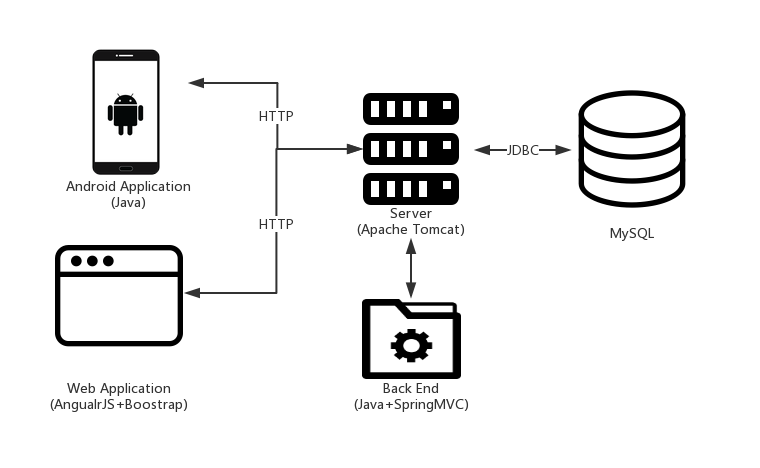
\includegraphics[width=4in]{figure/1}  	%插入的图,包括JPG,PNG,PDF,EPS等,放在源文件目录下
		\caption{Architecture Design of the Project}   %标签,用作引用
		\end{figure}
HTTP protocol will be used both for web application and Android application between server, and the token will be required for verification when two clients send HTTP request to the server. For the web application, Bootstrap and AngularJS will be used for front-end development, Java and Spring MVC will be applied to back-end development. For the Android application, its design and implementation will follow the Material Design. JDBC (Java Database Connectivity) will be used as the interface for the connection with MySQL database.

\subsection{Security Design}\label{3.3}
In order to prevent the divulgence of user information(username, password) by the network packet capture, RSA algorithm will be used for encrypt and decrypt user information when user login. As shown in figure 2, before user login, client will get the public key by sending GET method to the server, 
\begin{figure}[h]%%图
		\centering  %插入的图片居中表示
		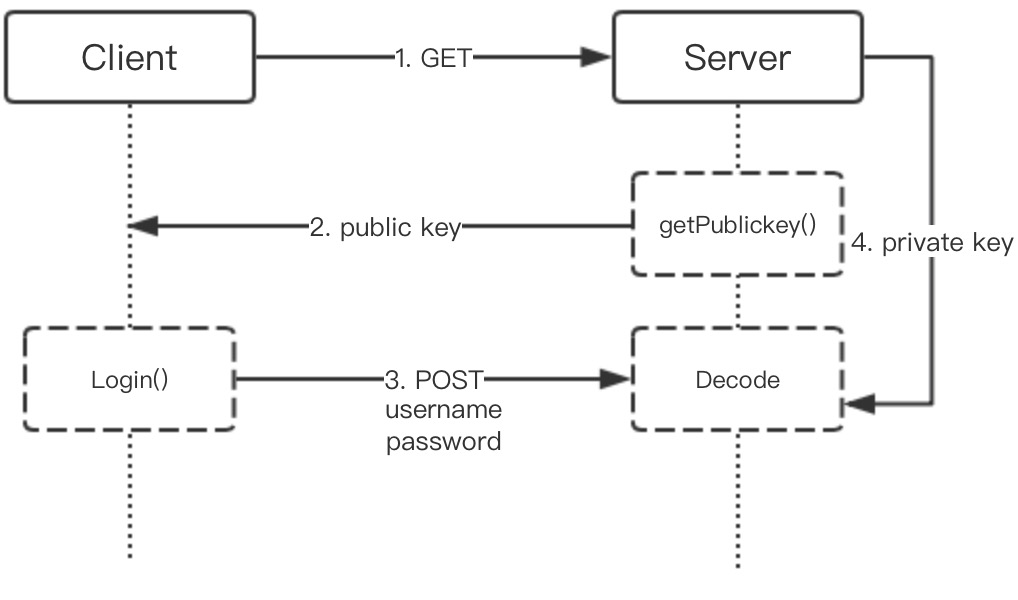
\includegraphics[width=4in]{figure/2}  	%插入的图,包括JPG,PNG,PDF,EPS等,放在源文件目录下
		\caption{Use RSA Algorithm for User Login }   %标签,用作引用
		\end{figure}
and the public key will be used to encrypt user information with the POST method. After server receiving the request, it will use the private key to decrypt the information.
\\
\\
As shown in figure 3, in order to verify users’ identities when 
\begin{figure}[h]%%图
		\centering  %插入的图片居中表示
		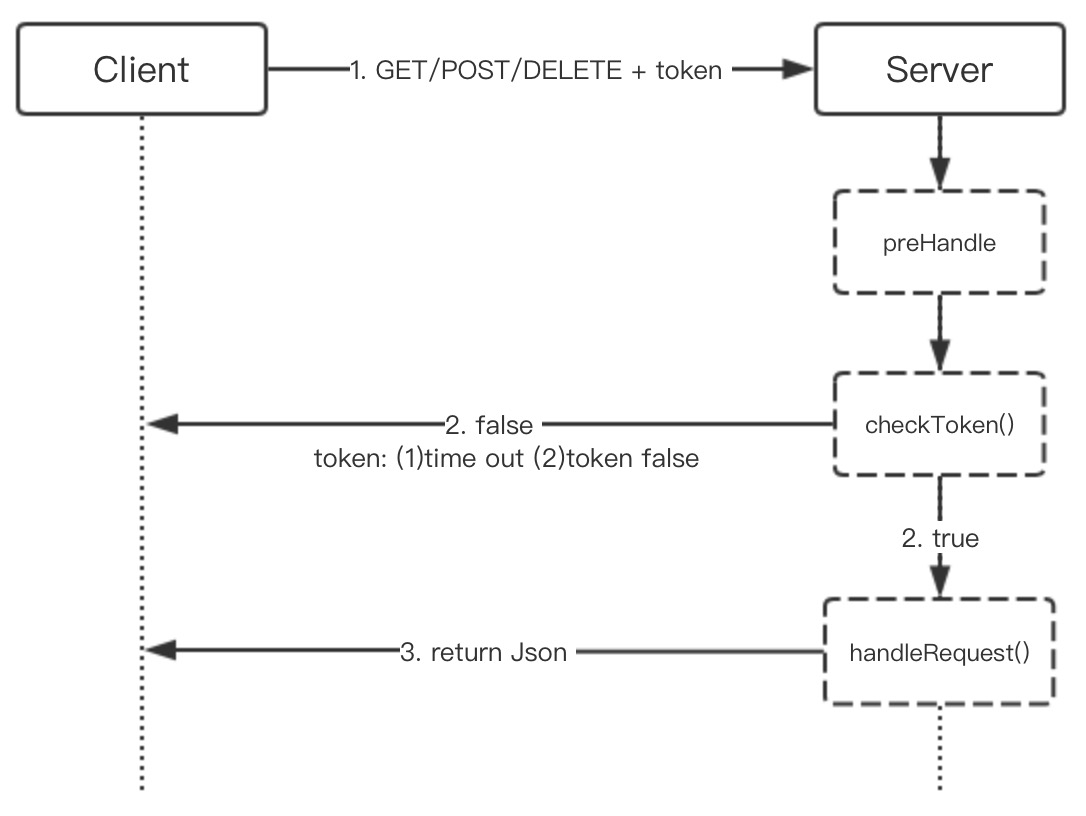
\includegraphics[width=4in]{figure/3}  	%插入的图,包括JPG,PNG,PDF,EPS等,放在源文件目录下
		\caption{Use Token for User Verification}   %标签,用作引用
		\end{figure}
they are using, a token will be required every time for clients while sending HTTP methods to the server. What’s more, the server will check the token before handle the HTTP request, and the token includes the identification of user and the expiration time of login.\\\\
What’s more, all the paths of files will be transform as Base64 encoded string, instead of transmitting them as clear text, which may be accessed without access permissions,and this plan of design shown as firgure 4.
\begin{figure}[h]%%图
		\centering  %插入的图片居中表示
		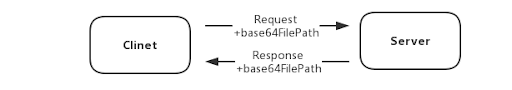
\includegraphics[width=4in]{figure/4}  	%插入的图,包括JPG,PNG,PDF,EPS等,放在源文件目录下
		\caption{File Paths are Base64 Encoded }   %标签,用作引用
		\end{figure}
\subsection{Conflict Resolution}\label{3.4}
when server has the file V, and it’s version is 0 we call it V0, and the if it’s version is 1 we call it v1.\\
\\
As the figure 5 shows that when the user1 and user2 modify the same file the someone upload earlier , the conflict will be appear.
\begin{figure}[h]%%图
		\centering  %插入的图片居中表示
		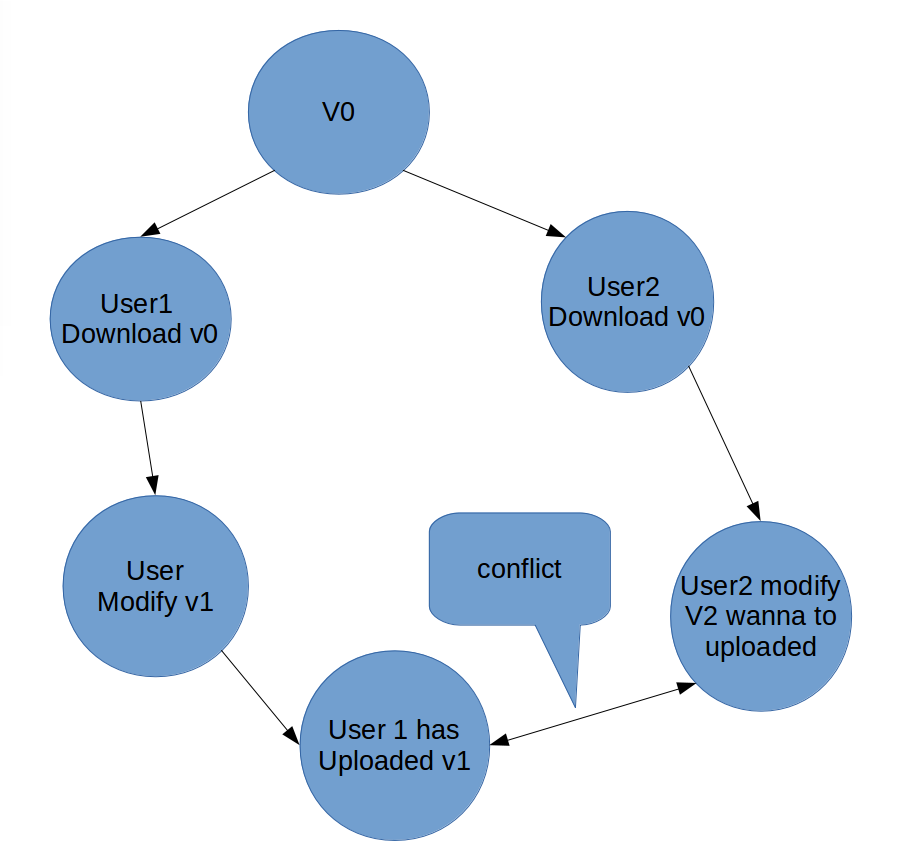
\includegraphics[width=2.5in]{figure/conflict}  	%插入的图,包括JPG,PNG,PDF,EPS等,放在源文件目录下
		\caption{When the conflict appear}   %标签,用作引用
		\end{figure}
		\\
Solution:
When user2 uploaded the new file V2, V2 will be compared with V0 and V1. As the way showed in the first problem to solve the image, text and other files, We use the different index to sort the V0,V1,V2. and then I will put the first into the New Version. Put the second into the Old Version. And discard the third.





\section{Implementation}\label{4}
\subsection{Back-End}\label{4.1}
The back-end side use Spring MVC as the web framework to handle the HTTP requests from clients, which is simple and clear by using MVC(Model, View, Controller) architectural pattern to make lower coupling between parts. However, since this project is not a only web application but both works for Android devices, the part of View will be separated out and will be implemented by web application and Android application individually.\\
\\
Here is the typical procedure how Spring MVC handle the HTTP requests in this project as figure 6:
\begin{figure}[h]%%图
		\centering  %插入的图片居中表示
		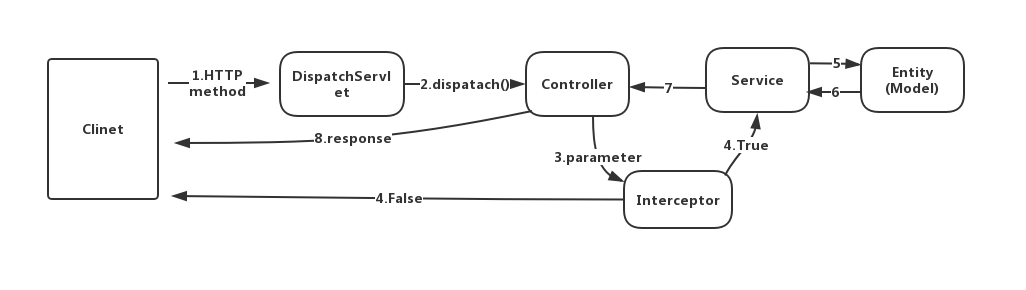
\includegraphics[width=4in]{figure/5}  	%插入的图,包括JPG,PNG,PDF,EPS等,放在源文件目录下
		\caption{Procedure of Spring MVC handle HTTP request}   %标签,用作引用
		\end{figure}
\\
There is a description of the code fragment when client side want to get a whole file list by sending GET methods http.get(“api/files/”):
\\
\\
1) The DispatchServlet will dispatch this request to the “FileController.java” because of the Spring MVC annotation “@Controller” and “@RequestMapping("/files")”:
\begin{figure}[h]%%图
		\centering  %插入的图片居中表示
		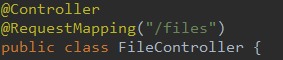
\includegraphics[width=3in]{figure/first}  	%插入的图,包括JPG,PNG,PDF,EPS等,放在源文件目录下
		\caption{class FileController}   %标签,用作引用
		\end{figure}
	\\
2)According to the Get methods http.get(“api/files/”,token), it a default get method without any path varivable, so the controller will call the 
\begin{figure}[h]%%图
		\centering  %插入的图片居中表示
		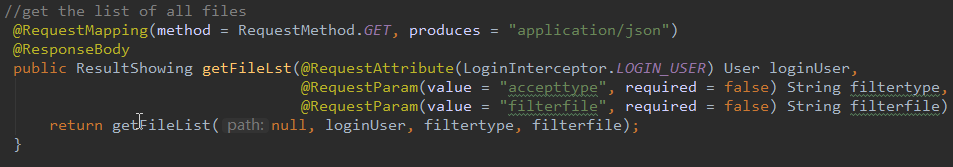
\includegraphics[width=5in]{figure/second}  	%插入的图,包括JPG,PNG,PDF,EPS等,放在源文件目录下
		\caption{function getFileLst()}   %标签,用作引用
		\end{figure}
function “public ResultShowing getFileLst(……)” by annotation “@RequestMapping(method = RequestMethod.GET, produces = "application/json")”
\\
\\
3)Until now, the function “getFileLst()” will not be called directly since the LoginInterceptor will check the parameter first
\begin{figure}[h]%%图
		\centering  %插入的图片居中表示
		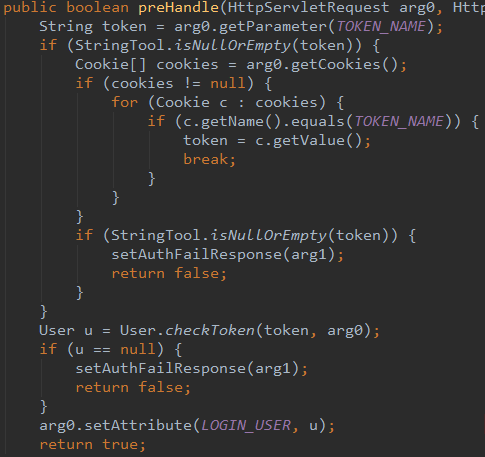
\includegraphics[width=3in]{figure/third}  	%插入的图,包括JPG,PNG,PDF,EPS等,放在源文件目录下
		\caption{function preHandle()}   %标签,用作引用
		\end{figure}
If the parameter “token” is not valid or expired, it will call “ setAuthFailResponse()” and return false, which will send error response back to the client.
\begin{figure}[h]%%图
		\centering  %插入的图片居中表示
		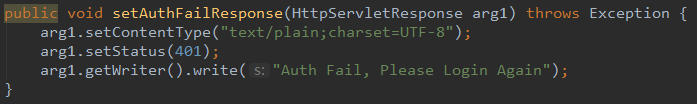
\includegraphics[width=4in]{figure/third2}  	%插入的图,包括JPG,PNG,PDF,EPS等,放在源文件目录下
		\caption{function setAuthFailResponse()}   %标签,用作引用
		\end{figure}
\\
\\
\\
\\
\\
\\
\\
\\
\\
\\
\\
4)If the parameter “token” is valid and not expired, it will go back to call the function “getFileLst()” successfully, and it will return the type of class “ResultShowing” to the client. However, before it return, the third party library “jackson” will encapsulate this class “ResultShowing” into the former of JSON(JavaScript Object Notiation) to the clinet.	
\\
\\
Except how handle HTTP requests, the most significant implementation in back-end will be the file operations by using “File.class” in the package “java.io”. After users register their account successfully, it will create two folders for users automatically, and the level will be “Username->Default”.\\\\ 
\begin{figure}[h]%%图
		\centering  %插入的图片居中表示
		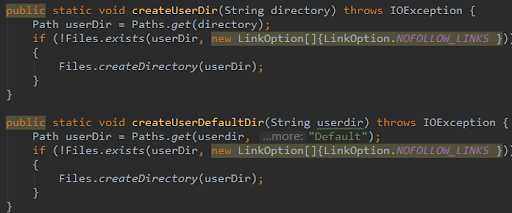
\includegraphics[width=4in]{figure/except1}  	%插入的图,包括JPG,PNG,PDF,EPS等,放在源文件目录下
		\caption{function createUserDir() and createUserDefaultDir()}   %标签,用作引用
		\end{figure}
\\
\\
\\
What’s more, after user upload file, back-end will use the method provided by library “commons-fileupload”, which is provides a simple and flexible means of adding support for multipart file upload functionality to servlets and web applications. In this project, we use it to get the file from the request:\\
\begin{figure}[h]%%图
		\centering  %插入的图片居中表示
		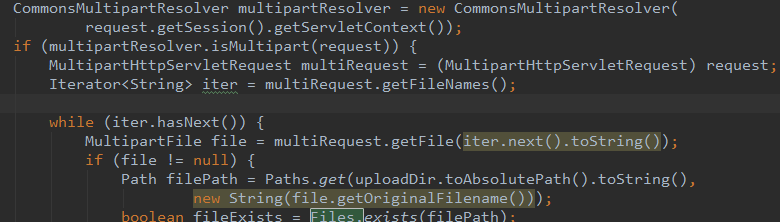
\includegraphics[width=4in]{figure/except2}  	%插入的图,包括JPG,PNG,PDF,EPS等,放在源文件目录下
		\caption{class fileUpload()}   %标签,用作引用
		\end{figure}\\
Delete file will use the “Files.delete()” directly:
\begin{figure}[h]%%图
		\centering  %插入的图片居中表示
		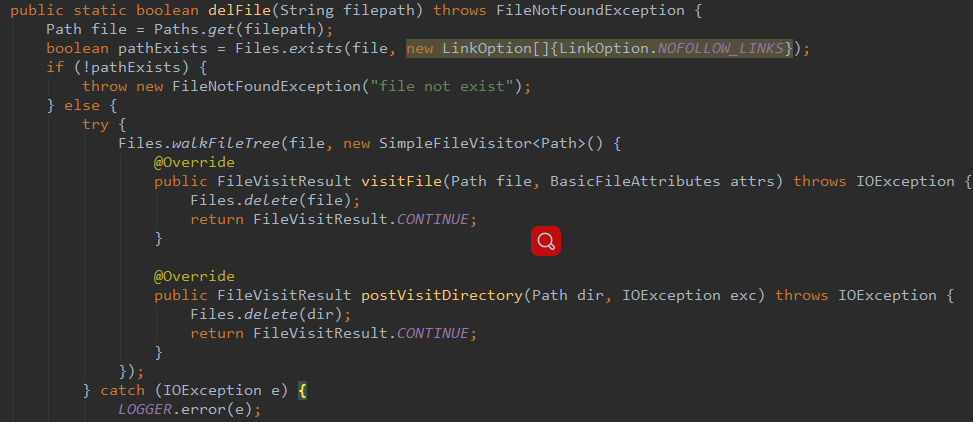
\includegraphics[width=4in]{figure/except3}  	%插入的图,包括JPG,PNG,PDF,EPS等,放在源文件目录下
		\caption{function delFile()}   %标签,用作引用
		\end{figure}
\\
\\
\\
\\
\\
\\
\\
\\
\\
\\
\\
\\
\\
The logic of rename file will check if the new name is the same as the old one before replace it:
\begin{figure}[h]%%图
		\centering  %插入的图片居中表示
		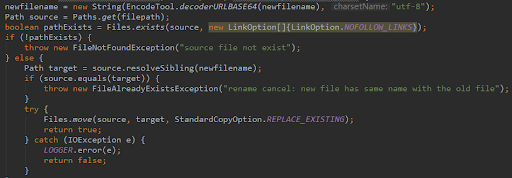
\includegraphics[width=4in]{figure/except4}  	%插入的图,包括JPG,PNG,PDF,EPS等,放在源文件目录下
		\caption{function moveFile()}   %标签,用作引用
		\end{figure}
\paragraph{Library use:}~{}
\newline
The project use Maven as the project management and comprehension tool, so all the library uses are in the “pom.xml” file.\\\\
1. Jackson:\\
Jackson is a JSON parser for Java, the project use it to cover Java class into JSON when return response to the client\\\\
2. Log4j:\\
Log4j is a Java logging tool to track and record the output console, and there are all levels we are using to classify the different outputs “All < Trace < Debug < Info < Warn < Error < Fatal < OFF”.\\\\
3. commons-fileupload:\\
Commons-fileupload can parse the request and make the results available in a manner easily used by the Java web developer.\\\\
4. spring-webmvc\\
Spring-webmvc provides a Java framework which is used to build Java web applications by the Model-View-Controller design pattern, and it also contains all the basic features of a core spring framework like Inversion of Control, Dependency Injection.

\subsection{Conflict Resolution}\label{4.2}
\subsubsection{Four implementation tool}\label{4.2.1}
\paragraph{Compare two image file, and get the similarity rate of the picture}~{}
\newline
\\
GetPX function:\\
This function is used to get the binary value of a image, the then
if the image has been changed , the binary value of the image will be different.
\begin{figure}[h]%%图
		\centering  %插入的图片居中表示
		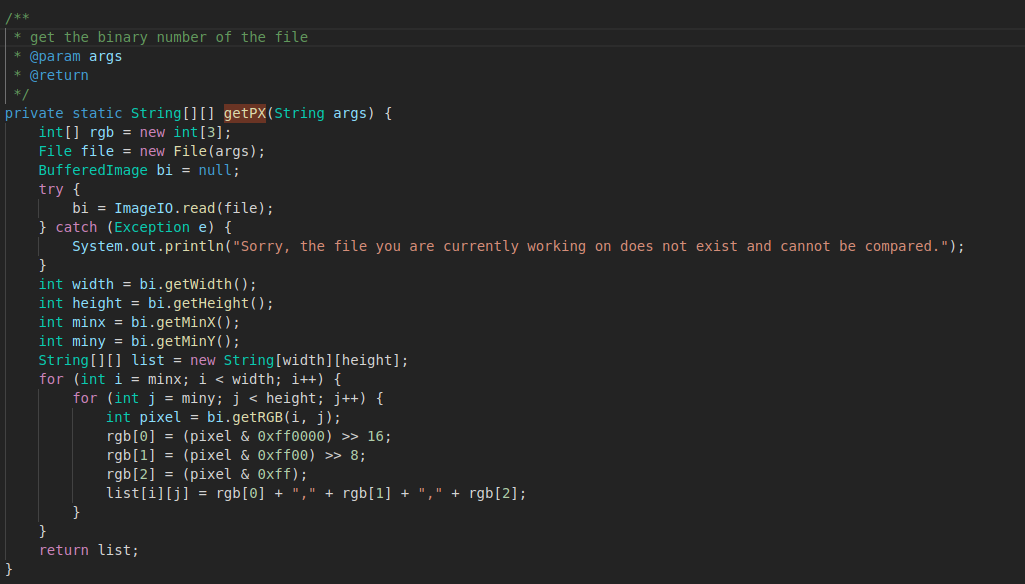
\includegraphics[width=4in]{figure/4211}  	%插入的图,包括JPG,PNG,PDF,EPS等,放在源文件目录下
		\caption{Convert the image to binary number}   %标签,用作引用
		\end{figure}
\\Compare image function:\\
This function is use to compare the similarity of two picture. The input are the path of two image path, and the output are the ”number of the similar pixels”,”number of dissimilar pixels”,”similarity rate”.
\begin{figure}[h]%%图
		\centering  %插入的图片居中表示
		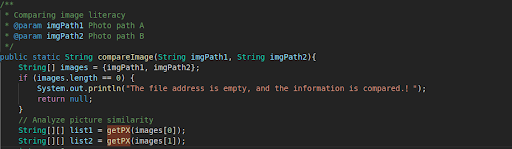
\includegraphics[width=4in]{figure/4212}  	%插入的图,包括JPG,PNG,PDF,EPS等,放在源文件目录下
		\caption{Compare the image}   %标签,用作引用
		\end{figure}
The middle is the function implementation process. \\
The return of the function is below
\begin{figure}[h]%%图
		\centering  %插入的图片居中表示
		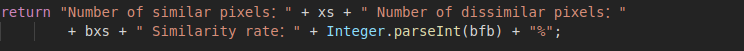
\includegraphics[width=4in]{figure/421333}  	%插入的图,包括JPG,PNG,PDF,EPS等,放在源文件目录下
		\caption{The result of compare image}   %标签,用作引用
		\end{figure}
\paragraph{Compare two text file, get difference in number of characters.}~{}
\newline
\begin{figure}[h]%%图
		\centering  %插入的图片居中表示
		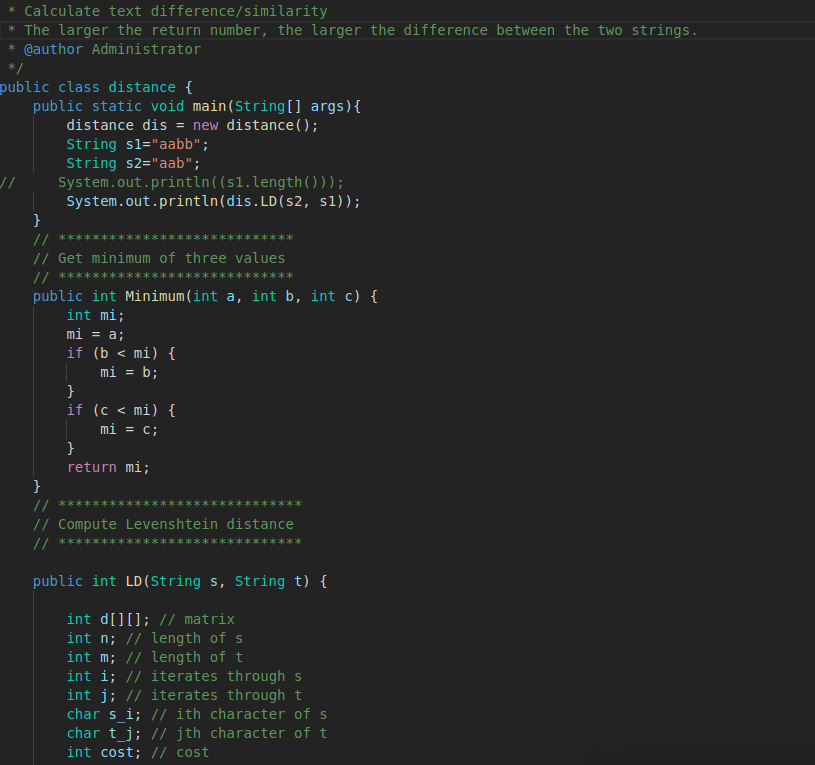
\includegraphics[width=2.5in]{figure/4221}  	%插入的图,包括JPG,PNG,PDF,EPS等,放在源文件目录下
		\caption{Use Levenshtein distance to compare the test file}   %标签,用作引用
		\end{figure}
\\\\\\\\
The class distance:\\
The input of the function is the content of the text file\\
The output of the function is the difference between two files
\\\\
Our team mainly used the Levenshtein  distance algorithm to calculate the main difference of the text file. The result of the Levenshtein  distance is bigger the difference of the two files
\paragraph{Other file compare}~{}
\newline
\begin{figure}[h]%%图
		\centering  %插入的图片居中表示
		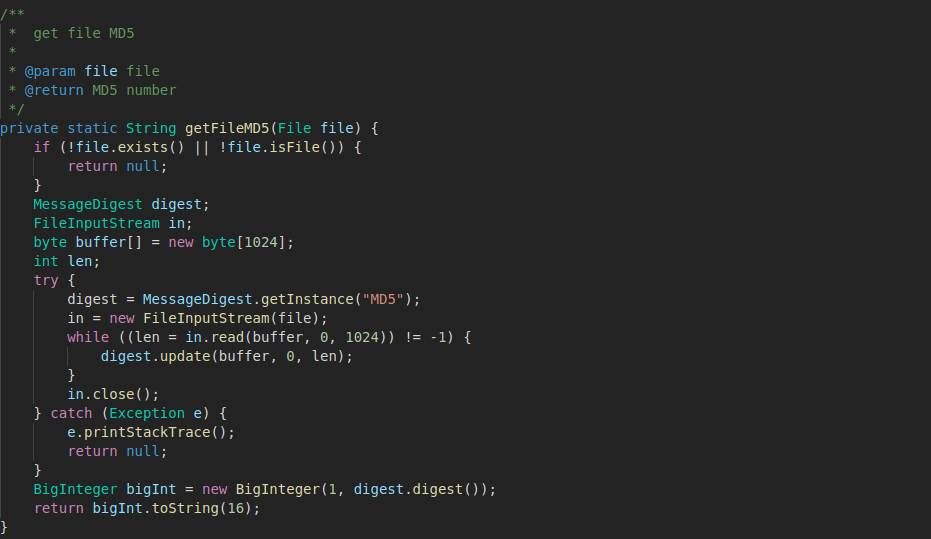
\includegraphics[width=2.5in]{figure/4231}  	%插入的图,包括JPG,PNG,PDF,EPS等,放在源文件目录下
		\caption{Use the MD5 value to compare the file same or not}   %标签,用作引用
		\end{figure}
Our team use the value of the MD5 of the file to compare two file whether they are same or not.\\\\
MD5 value is a good way to compare the two file, if the file has been modified the MD5 value will be changed.
\begin{figure}[h]%%图
		\centering  %插入的图片居中表示
		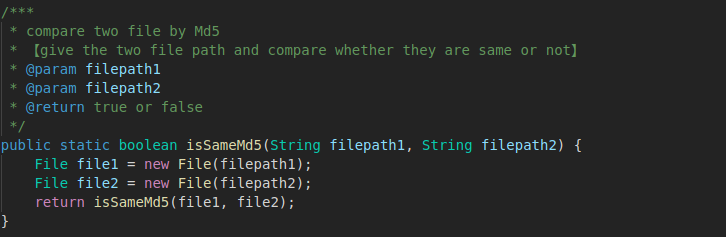
\includegraphics[width=4in]{figure/4232}  	%插入的图,包括JPG,PNG,PDF,EPS等,放在源文件目录下
		\caption{The function of the compare file by MD5}   %标签,用作引用
		\end{figure}
\\\\\\\\\\\\\\\\
Since we use the file path to save it on the server. So we take the file path as an incoming parameter, and give the return of true or false as the result of the file compare
\paragraph{Change the file path of folder}~{}
\newline
\begin{figure}[h]%%图
		\centering  %插入的图片居中表示
		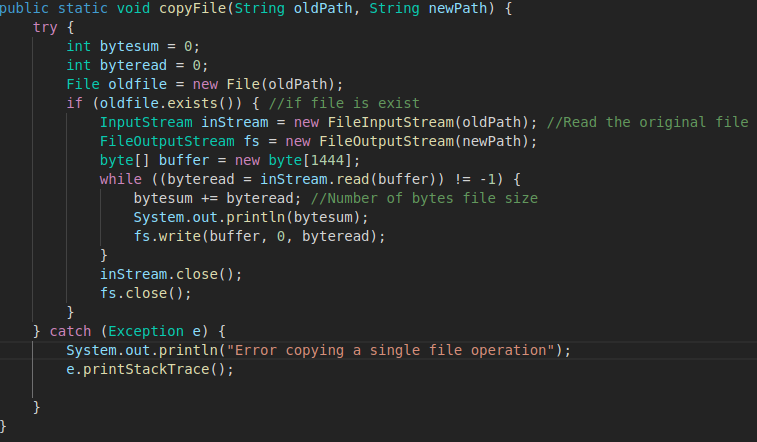
\includegraphics[width=4in]{figure/4241}  	%插入的图,包括JPG,PNG,PDF,EPS等,放在源文件目录下
		\caption{Change the file path of the folder}   %标签,用作引用
		\end{figure}
The copyFile function is used to copy file content according to the file path, and move the file to the specified folder.
\subsubsection{The implementation of the main function
}\label{4.2.1}
\paragraph{Solve the version control problem}~{}
\newline
\begin{figure}[h]%%图
		\centering  %插入的图片居中表示
		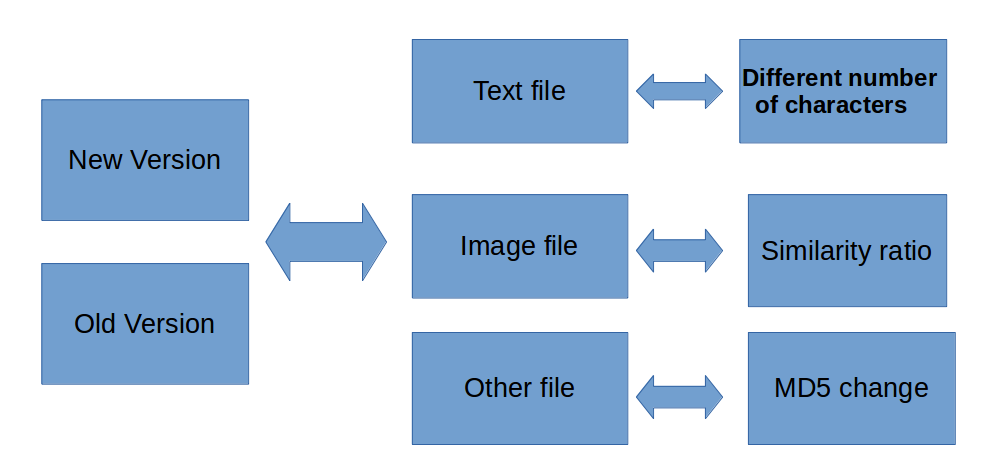
\includegraphics[width=4in]{figure/ffirst}  	%插入的图,包括JPG,PNG,PDF,EPS等,放在源文件目录下
		\caption{Version control}   %标签,用作引用
		\end{figure}
There are two folder in the server one is “New Version”, and the other one is “Old Version” . And the save the first version and second version. 
\\\\
\paragraph{When the third verison is coming:}~{}
\paragraph{If the file is text file}~{}
\newline
I will compare the file with the second version of the first version, and then use the Levenshtein distance algorithm to calculate the file characters difference. The result is positive or negative value.
Then sort by the result of the comparison to get the first second and third. And then I will put the first into the New Version. Put the second into the Old Version. And discard the third.
\paragraph{If the file is image file}~{}
\newline
I will compare the file with the second version of the first version, and then use the binary value of the image to calculate the file pixels difference. The result is similarity ratio.
Then sort by the result of the comparison to get the first second and third. And then I will put the first into the New Version. Put the second into the Old Version. And discard the third.
\paragraph{If the file is other file}~{}
\newline
I will compare the file with the second version of the first version, and then use the MD5 value of the file to determine the file difference. The result is ture or false.
Then sort by the result of the comparison to get the first second and third. And then I will put the first into the New Version. Put the second into the Old Version. And discard the third.
\subsubsection{Flow chart of the whole implementation}\label{4.2.3}
\begin{figure}[h]%%图
		\centering  %插入的图片居中表示
		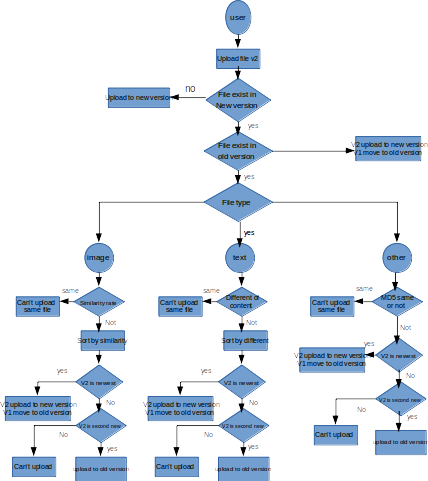
\includegraphics[width=4in]{figure/blur}  	%插入的图,包括JPG,PNG,PDF,EPS等,放在源文件目录下
		\caption{Flow chart of the whole implementation
}   %标签,用作引用
		\end{figure}
\subsection{Web Application}\label{4.3}
The main and significant implementation of web application except the common web design and implementation by HTML and CSS will be how to send the HTTP request to the server and how to implement the RSA algorithm and token in the security design.\\\\
The web application use AngularJS to handle the the business logic tier. It provides API “\$http” help us to send the HTTP methods simply:
\begin{figure}[h]%%图
		\centering  %插入的图片居中表示
		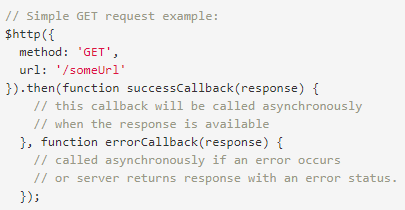
\includegraphics[width=4in]{figure/white}  	%插入的图,包括JPG,PNG,PDF,EPS等,放在源文件目录下
		\caption{implementation GET by AngularJS}   %标签,用作引用
		\end{figure}
\\After web client get the public key from the server, it will use it to create token as well as use it to encrypt user information, and the token will be store in the cookie by browser and may will be used for the server side:
\begin{figure}[h]%%图
		\centering  %插入的图片居中表示
		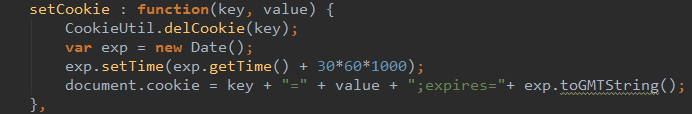
\includegraphics[width=4in]{figure/white2}  	%插入的图,包括JPG,PNG,PDF,EPS等,放在源文件目录下
		\caption{function setCookie() in "cookie.js"}   %标签,用作引用
		\end{figure}
\paragraph{Library use:}~{}
\newline
1.AngularJS:\\
AngularJS iis a structural framework for dynamic web application, which provides a simple way for date binding, DOM control structures for repeating, showing and hiding DOM fragments.\\\\
2.jsencrypt.js\\
“jsencrypt.js” is used to encrypt the username and password by RSA algorithm before sending them to the server:\\\\
3.base-64.min.js\\
“base-64.min.js” is used to encode the file name and file path by Base encoding, in case of leak location of the user’s file.\\\\
4.bootstrap.min.js\\
Bootstrap is a CSS framework which provide many built-in style by using <class=”style name”> easily.\\\\
5.clibboard.min.js\\
It’s quick copy and paste tool for user when they need to share file by send link and password to others.

\subsection{Android Application}\label{4.4}


\subsubsection{Android Introduction}\label{4.3.1}
Initially, we choose Android Studio as our development tool, because it would be easier for us to implement all function into our app. However, we decided to choose Android as our only target mobile platform since Android has almost 88\% market share nowadays[3]. Therefore, Java was used to build our Android Application, which is quite  the same as the logic of web application. In addition, we also use some external libraries


\subsubsection{Android Implementation}\label{4.3.2}
Basically, we implemented our app using APIs from back-end, and we also tried to move all functions from web application into mobile app. As the first step of Android design process, UI design plays an important part of it, and we decided to implement a colorful login page and simple style mainpage. Secondly, we jumped into coding part and followed all logic we designed in our server. For example,we implemented the function of login user at 'WelcomeActivity' by sending GET and POST methods to the web server, and received all datas of user from server. Moreover, as our main function, uploading and downloading are also implemented into our mobile app. Last, OkHttp is an external library, which we  used as a tool to POST request into server. However, there are some difference between mobile app and desktop application. Users would not be able to move files through mobile app, and there are also some differences in showing information between mobile and desktop.


\subsubsection{Android Testing}\label{4.3.3}
The project includes 2 testing target. The first target contains unit tests for testing various functionality of the project. The second is a instrumentation testing target, which will test all UI and its logic.

\subsection{Testing}\label{4.4}
\subsubsection{Unit testing}\label{4.4.1}
In testing, we used JUnit test framework to help us in validation our methods for functionality. As our known, A JUnit test is a method contained in a class which is only used for testing. After creating the test class, we need to annotated it with the @Test annotation to define it as a test method. This method executes the code under test. In the testing implementation phase, we tested 16 main class from back-end code including service, controller, entity and tool, etc. 
\begin{figure}[h]%%图
		\centering  %插入的图片居中表示
		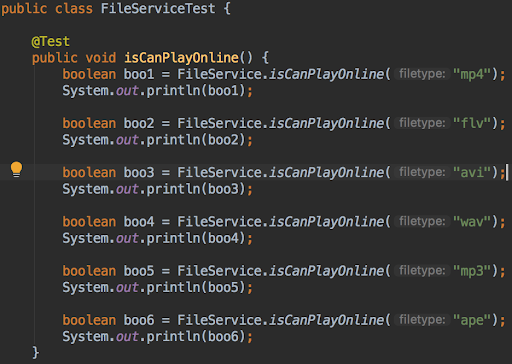
\includegraphics[width=3.5in]{figure/n}  	%插入的图,包括JPG,PNG,PDF,EPS等,放在源文件目录下
		\caption{Test Class for FileService}   %标签,用作引用
		\end{figure}
According for different logic and function, we recalled the method written in the code under test by using different valid and invalid parameters. Due to each input correspond to different output, we printed the return values of each method and judged its reasonability. If the return value is what we expect, than it is right. Take an "FileServiceTest" class as an example, as shown in figure 11.
In order to test if it could play the audio file with different formats well, we compiled several input parameters such as mp4, flv, avi, wav, mp3, ape etc. And we obtained the following return values, as shown in figure 12. 
\begin{figure}[h]%%图
		\centering  %插入的图片居中表示
		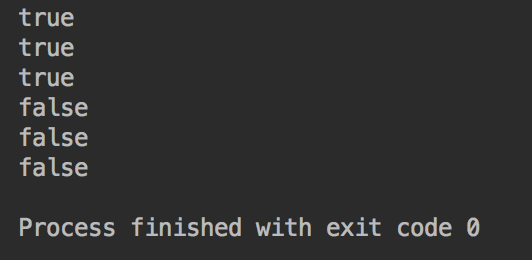
\includegraphics[width=2in]{figure/n1}  	%插入的图,包括JPG,PNG,PDF,EPS等,放在源文件目录下
		\caption{Return values in executing the test class}   %标签,用作引用
		\end{figure}
The first three returns are true and false else representing the first three audio file formats are what we supported and the rests are unsupported, which is what we expected.

\subsubsection{Black box testing }\label{4.4.2}
Black-box testing is a method of software testing that examines the functionality of an application without peering into its internal structures or workings. 
\newcommand{\tabincell}[2]{\begin{tabular}{@{}#1@{}}#2\end{tabular}} 
\begin{table}[h]
\caption{Test case of black box testing.} 
\begin{tabular}{|p{100pt}|p{130pt}|p{130pt}|}
\hline
Function           & Test case                                                                                     & Test Result                                                              \\
\hline
File upload        & Click the Upload button and Select File dialog box popup, and then select the file.           & After the upload is completed, website prompts that upload is successful \\
\hline
File download      & Left-click on the file in the file list and select Download in the middle of the pop-up menu. & File is successfully downloaded.                                         \\
\hline
File/folder create & Left-click the Upload File button and select a file in the file list                          & File is successfully created.                                            \\
\hline
File/Folder delete & Left-click the file and select Delete in the middle of the pop-up menu.                       & File is successfully deleted. \\                                          
\hline
\end{tabular}
 
\end{table}
This method of test can be 
applied virtually to every level of software testing: unit, integration, system and acceptance. It is sometimes referred to as specification-based testing(Table 1).

\subsubsection{Stress testing}\label{4.4.3}
In maintenance work, stress testing is an essential task. For example, before a website is launched, how much traffic it can afford and how well it performs in large traffic situations will directly affect the user experience. However, there is a commonality in the stress test; that is, the results of the stress test and the actual load results will not be the same. Even if the stress test work is done well, there is no guarantee that 100\% and the online performance indicators are the same. Faced with these problems, we can only try to find ways to simulate. Therefore, stress testing is vital. With this data, we can be quite aware of our platform for maintenance. Webbench is a well-known website stress testing tool developed by Lionbridge Corporation.
We use webbench to complete our stress test. We simulate four situations as follow four figures. The results show that our ONEBOX could perform well in a stress situation.
\begin{figure}[h]%%图
		\centering  %插入的图片居中表示
		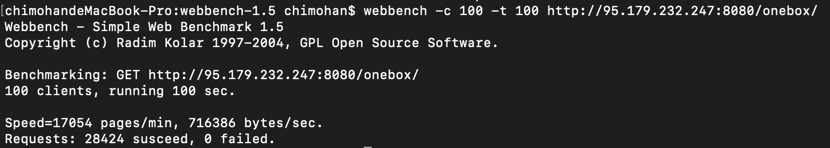
\includegraphics[width=4in]{figure/4331}  	%插入的图,包括JPG,PNG,PDF,EPS等,放在源文件目录下
		\caption{100 clients, running 100 seconds}   %标签,用作引用
		\end{figure}
\begin{figure}[h]%%图
		\centering  %插入的图片居中表示
		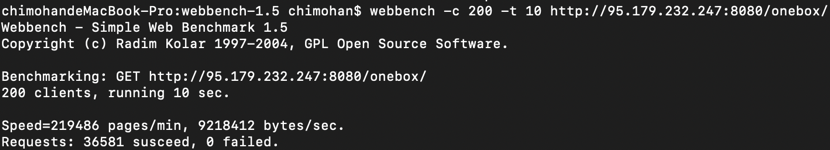
\includegraphics[width=4in]{figure/4332}  	%插入的图,包括JPG,PNG,PDF,EPS等,放在源文件目录下
		\caption{200 clients, running 10 seconds}   %标签,用作引用
		\end{figure}
\begin{figure}[h]%%图
		\centering  %插入的图片居中表示
		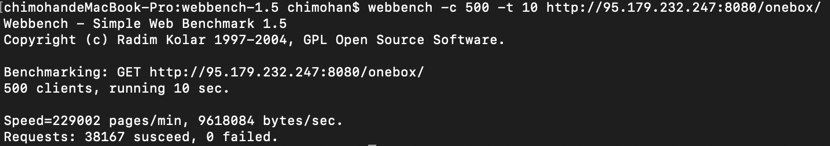
\includegraphics[width=4in]{figure/4333}  	%插入的图,包括JPG,PNG,PDF,EPS等,放在源文件目录下
		\caption{500 clients, running 10 seconds}   %标签,用作引用
		\end{figure}
\begin{figure}[h]%%图
		\centering  %插入的图片居中表示
		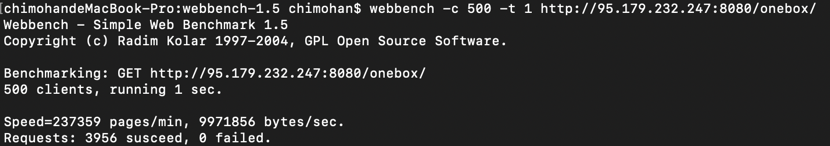
\includegraphics[width=4in]{figure/4334}  	%插入的图,包括JPG,PNG,PDF,EPS等,放在源文件目录下
		\caption{500 clients, running 1 second}   %标签,用作引用
		\end{figure}
\section{Team work}\label{5}
\subsection{Organization}\label{5.1}
We decided to split our team into three sub-team, which are front-end, back-end and mobile based on members' preferences and abilities. We believe this method would greatly improve our efficiency and put everyone into right place. GitHub is the tool that we used for our project, and we also used SourceTree as our tool to keep all updates and merge different branches. During last two weeks of this semester, our major jobs were wrapping all coding and preparing all documents and presentation. As for the coding part, we did some optimizations for our project for example to accelerating the loading time for mobile app and finished all unit tests. In the last week, we met four times in order to finish all documents and rehearsed the presentation. There are some improvements can be made for team working. First of all, we should put each task more specific into everyone' lists. Secondly, communication can also be improved, because there is some miscommunication happened during this project for example some members did repeatable jobs.
\subsection{Meeting}\label{5.2}	
At the beginning, our group decided to meet twice a week in order to discuss coding or design problems. However, due to the conflicts of timetable for each group members., we decided to meet once a week and have some online meetings by using WeChat. There are three significant processes during this development. Firstly, we took two weeks in analysis and designed our project. During that time, our team had a new member, and we built a group chat in order to facilitating group work. Jumped into a next phase of our project, we started coding part of our project. Moreover, we still meet once a week to discuss all problems that we meet in this week and try to get a solution for those problems (every Thursday afternoon, bush house 6th floor), and we still have online meetings regularly.

\subsection{Strength}\label{5.3}	
Each member of our team has carefully invested their own efforts and worked together to ensure the successful implementation of the project objectives. Our group achieved the following key points:
(1) A clear understanding of the project objectives.
(2) Clear expectations for each member's roles and responsibilities.
(3) Goal orientation.
(4) High degree of cooperation and mutual assistance.
(5) Highly trusted.
To effectively manage time, each team member must define weekly goals, develop a schedule each day, and focus on completing the day's plan. Every member of our team is dedicated to this project and looks forward to the successful implementation of the project.
\subsection{Weakness}\label{5.4}
Facing new teams, technical unfamiliarity, unclear needs, and short project durations, we met lots of difficulties. From the beginning to the delivery of the final version, the problems and risks coexist, so we dare not to relax and scorn. 
The project team has insufficient experience, relevant research, and development experience, so our work was stagnant at the beginning of the project. Here are the issues we encountered at each stage of the project.

\section{Evaluation}\label{6}
In this section, we will evaluate our project objectively. we will mainly discuss the advantages and disadvantages of this project.
We basically complete the file synchronization system, users can access their file management system from the desktop and Android application. Users need to register an individual account before using the system and then it can log in to the system and use it. The system mainly includes the following functions: user registration/login function, file upload/download function, file/folder deletion and renaming function, file movement function, file sharing function. We have also developed version control and file comparison functions based on these basic functions.
\\
\\
Below table outlines the completion of each function of the project:

\begin{table}[h]
\caption{Project completion}  
\begin{tabular}{|l|l|l|}
\hline
Function                    & Desktop completeness & Android completeness \\
\hline
Login                       & completed            & completed            \\
\hline
Register                    & completed            & completed            \\
\hline
Upload file                 & completed            &completed                      \\
\hline
Download file               & completed            &completed                      \\
\hline
Delete file/folder          & completed            &completed                      \\
\hline
Rename file/folder          & completed            &completed                      \\
\hline
Move file                   & completed            &uncompleted                      \\
\hline
Share file                  & completed            &uncompleted                      \\
\hline
Version control             & completed            &completed                      \\
\hline
File comparison             & completed            &completed                      \\
\hline
Browse picture/video online & completed            & uncompleted\\
\hline 

\end{tabular}

\end{table}

\subsection{Advantage of the project}\label{6.1}
\subsubsection{The front-end design}\label{6.1.1}
The first thing must be mentioned is our front-end development part. We use the bootstrap framework for front-end development which provides a simple and unified solution for developers to create interfaces and includes powerful built-in components that are easy to customize. At the same time, our front-end page is simple and artistic, and the UI is user-friendly.

\subsubsection{Basic back-end function}\label{6.1.2}
Another advantage is our login function which allows authorized users to access the file system, and it ensure the secure of this system. When user logs in, database will be checked to find whether it matches between the username with the password. If there is no match, the user will be notified that the password is incorrect.
\\\\
We have also successfully implemented a feature that allows users to modify the file name on the database which allows people to save conflict files with a separate name without wanting to overwrite the main file.

\subsubsection{Advanced back-end function}\label{6.1.3}
Based on the full implementation of the basic functions, this system also implements version control function. When different users make different changes to the same original file and upload the same document to the server, the system uses a mature algorithm to control the file version in the system.
\\\\
Besides, the file comparison function is also a highlight of this system and this function collaborate with the version control function. When different user changes the same file and upload it, this system will compare the different version of this file. The main type of file includes image file and text file.
\\\\
User can browse pictures and video online when using this system. This function makes it more efficient because the user do not need to download the image and video file and check it online, it reduce the time so much.
\subsubsection{Security}\label{6.1.4}
It uses RSA algorithm when user logging into the system, the server will generate a key pair (public key and key). When the user logs in, it will be transmitted to the server after the public key is encrypted. The server will decrypt the encrypted data with the key. Ensure that users and passwords are not exposed even if they are captured when sending HTTP requests. After the login is successful, all HTTP requests which includes GET, POST, DELETE, HEAD requests need to be carried with a token which carries the expiration time and be sent to the server for verification. Besides, all paths are base64 encrypted when displayed on the front-end.500 clients, runnin

\subsection{Disadvantage of the project}\label{6.2}
\subsubsection{Android unfinished}\label{6.2.1}
Due to the time allocation is not reasonable enough, the some functions of android application are not complete. The uncompleted part of Android application includes these functions: Delete file, Move file and Share file.

\subsubsection{Online file edit}\label{6.2.2}
Another disadvantage of our system is that files cannot be edited directly in the system. This means that if a user needs to modify a file, this user must download it to modify.

\subsubsection{Unreasonable time allocation}\label{6.2.3}
Because neglecting the difficulty of this project at the initial stage, we began to develop it a little bit late, so the time allocation is not very reasonable. At the final stage of our project, everyone has large amount of work to do in a very short time, and everyone feel so stressed. This experience remind us that we should always prepare in advance.
\section{Peer assessment}\label{7}
\begin{table}[h]
\begin{tabular}{|l|l|l|}
\hline
Group Member & Student Number & Point \\
\hline
Tehao Ye     & 1826930        & 31    \\
\hline
Zhihao Zhu   & 1834878        & 13    \\
\hline
Jiawei Zhou  & 1819642        & 12    \\
\hline
Yibo Liu     & 1839502        & 11    \\
\hline
Yankai Chen  & 1877520        & 11    \\
\hline
Mohan Chi    & 1866550        & 11    \\
\hline
Jiawei Ding  & 1829975        & 11 \\
\hline  
\end{tabular}
\end{table}
\bibliographystyle{plain}
\bibliography{ExampleReferenceFile}
[1] (n.d.). Retrieved from https://www.aomeitech.com/cloud-storage/what-is-the-difference-between-dropbox-and-onedrive-0326.html
\\{}\\{}
[2] Nick. (n.d.). Dropbox vs. Google Drive vs. OneDrive: Which is Best? Retrieved from https://blog.tcitechs.com/blog/dropbox-vs-google-drive-vs-onedrive
\\{}\\{}
[3] Mobile OS market share 2018. (n.d.). Retrieved from https://www.statista.com/
\\
statistics/266136/global-market-share-held-by-smartphone-operating-systems/




\end{document}
